\documentclass[a4paper, 11pt, final, garamond]{book}
\usepackage{cours-preambule}
\usepackage{pdfpages}

\raggedbottom

\makeatletter
\renewcommand{\@chapapp}{Travaux pratiques -- TP}
\makeatother

\let\SavedIndent\indent
\protected\def\indent{%
  \begingroup
    \parindent=\the\parindent
    \SavedIndent
  \endgroup
}
\setlength{\parindent}{0pt}

\begin{document}
\setcounter{chapter}{12}

\chapter{\'Etude d'un filtre passe-bas du premier ordre}
\section{Objectifs}

\begin{itemize}
    \item Apprendre à utiliser un dBmètre.
    \item Apprendre à déterminer rapidement une fréquence de coupure.
    \item Apprendre à mesurer un déphasage à l'oscilloscope.
    \item Apprendre à tracer un diagramme de Bode sur papier semi-log et
        papier millimétré.
\end{itemize}

\section{S'approprier}

\subsection{Méthode pour mesurer un déphasage -- rappel de cours}

\begin{wrapfigure}[16]{r}{0.45\textwidth}
\vspace{-20pt}
    \begin{center}
        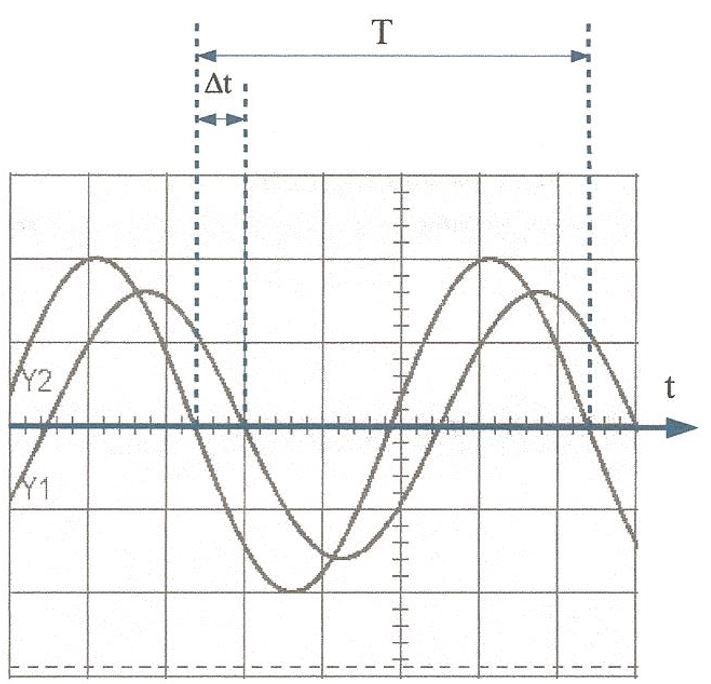
\includegraphics[width=0.4\textwidth]{dephasage}
    \end{center}
\vspace{-30pt}
\end{wrapfigure}

Le déphasage $\f$ entre deux signaux est un nombre appartenant à l'intervalle
$\left]-\pi~; \pi\right]$. Il se mesure grâce à l'oscilloscope. Pour toute
mesure, il faut que les deux signaux soient centrés afin de repérer l'écart
entre les «~passages par zéro~». Supposons $e(t) = E_{m} \cos(\w t)$ sur la voie
$Y_1$ et $s(t) = S_{m} \cos (\w t + \f)$ sur la voie $Y_2$ de l'oscillogramme
ci-contre. La détermination du déphasage se fait alors en deux étapes~:

\begin{itemize}
    \item \ul{Déterminer la valeur absolue de $\f$}~: pour cela, il faut placer
        les curseurs verticaux de manière à déterminer la période $T$ et le
        décalage $\Delta t$, puis $\left| \f \right| = 2 \pi \Delta t/T$ (en
        rad).
    \item \ul{Ensuite déterminer le signe de $\f$}~:
        pour cela, on cherche quelle courbe est en avance sur l'autre. Sur
        l'oscillogramme ci-contre, $Y_2$ est en avance par rapport à $Y_1$ car
        $Y_2$ s'annule en premier, donc $\f > 0$ (et inversement).
\end{itemize}


\subsection{Méthode pour mesurer un gain en dB}

Le gain se mesure grâce à un multimètre en fonction Volt alternatif (symbole
V$\sim$) puis dBmètre (bouton dB) pour activer la fonction dBmètre. Brancher le
multimètre sur l'entrée $e(t)$ du montage, appuyer sur «~rel~» une ou deux fois
jusqu'à ce que le multimètre affiche 0. On indique alors au multimètre que c'est
cette tension $e(t)$ qui sert de référence. Brancher ensuite le multimètre sur
la sortie $s(t)$. Il affiche directement le gain en dB.

\begin{brapp}{\includehand{-90}{0.8cm}}
    \centering
    \textbf{ATTENTION~: Il faut refaire le zéro relatif pour chaque fréquence.}
\end{brapp}

\subsection{Méthode pour tracer un diagramme de Bode}

Pour tracer le diagramme de Bode, il est nécessaire pour chaque fréquence de
déterminer~:
\begin{enumerate}
    \item le déphasage $\f$ de $s(t)$ par rapport à $e(t)$~;
    \item Le gain en dB.
\end{enumerate}

\section{Analyser}

\begin{minipage}{0.60\linewidth}
    Le montage étudié, schématisé ci-contre, est un circuit RC série alimenté
    par la tension $e(t) = E_{m} \cos(\w t)$. On pose $s(t) = S_{m} \cos (\w t +
    \f)$ la tension aux bornes du condensateur.
\end{minipage}
\hfill
\begin{minipage}{0.35\linewidth}
    \begin{center}
        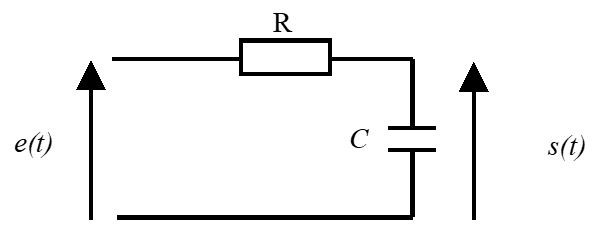
\includegraphics[width=\linewidth]{circuit}
    \end{center}
\end{minipage}

\begin{enumerate}[label=\sqenumi]
    \item Établir l'expression de la fonction de transfert.
    \item Déterminer le comportement asymptotique du filtre pour le gain et le
        déphasage.
    \item Déterminer l'expression de la fréquence de coupure $f_{c}$, puis la
        calculer pour $R=\SI{1,0}{k\Omega}$ et $C = \SI{0,10}{\mu F}$.

    \item Compléter le schéma avec les branchements de la carte Sysam permettant
        de visualiser simultanément $e(t)$ sur la voie $EA0$ et $s(t)$ sur la
        voie $EA1$ de l'oscilloscope.

    \item On souhaite éliminer toute composante continue des signaux observés,
        doit-on choisir le mode AC ou DC~? (vous pourrez faire une recherche sur
        internet ce que signifie mode AC et DC d'un oscilloscope).

    \item Si l'amplitude $E_{m}$ du signal d'entrée est représentée par
        $\num{2,8}$ carreaux, en supposant que la sensibilité verticale est la
        même sur les 2 voies, montrer que pour $f=f_{c}$ l'amplitude $S_{m}$ du
        signal de sortie correspond alors à 2 carreaux sur l'oscillogramme.
\end{enumerate}

\section{Réaliser}

\subsection{Etude rapide de comportement}

\begin{enumerate}
    \item Connecter la carte Sysam à l'ordinateur~;
    \item Ouvrir Oscillo5 (Programmes Physique-chimie $\rightarrow$ Eurosmart
        $\rightarrow$ Oscillo5)~;
    \item Alimenter votre filtre RC avec la sortie analogique SA1 de la carte
        Sysam
    \item Relever la tension $e(t)$ sur le canal EA0 et la tension $s(t)$ sur le
        canal EA1.
    \item Passer en mode Bode~;
    \item Afficher gain et phase~;
    \item Prendre une échelle log avec une étendue de fréquence cohérente avec
        la fréquence de coupure que vous avez préalablement déterminée~;
    \item Sélectionner EA0 en entrée~;
    \item Effacer acquisitions précédentes. choisir~: toutes~;
    \item Déclencher.
    \item Les diagrammes sont tracés de manière automatique. Pratique si on veut
        être rapide~!
\end{enumerate}

\subsection{Mesures pour le tracé du diagramme de Bode}

Il s'agit maintenant de faire un relevé fréquence par fréquence pour apprendre à
le faire «~à la main~». Prendre comme amplitude du signal d'entrée environ
$\SI{2}{V}$ (soit $\SI{4}{Vpp}$) en utilisant le mode GBF d'Oscillo5. Pour
\textbf{chaque} fréquence~:

\begin{enumerate}[resume]
    \item Mesurer le déphasage entre $s(t)$ et $e(t)$ à l'aide d'Oscillo5, comme
        indiqué dans S'approprier. Pour plus de facilité, utiliser les curseurs
        (en bas à droite du menu d'Oscillo5).
    \item Mesurer le gain en dB à l'aide du dBmètre, comme indiqué dans
        S'approprier.
    \item Faire varier les fréquences entre $\SI{100}{Hz}$ et $\SI{50}{kHz}$.
        Une échelle logarithmique de variation de la fréquence est pertinente et
        vous pourrez faire plus de mesures autour de la fréquence de coupure
        $f_{c}$ précédemment établie.
\end{enumerate}

\begin{enumerate}[label=\sqenumi, start=7]
    \item  Regrouper les valeurs dans un tableau faisant apparaître $f$ (en Hz)
        / $G_{\rm dB}$ / $\abs{\Delta t}$ (en s) / $\abs{\f}$ (en rad) /
        $\f$ (en rad).
\end{enumerate}

\section{Valider et conclure}

\begin{enumerate}[label=\sqenumi, resume]
    \item Tracer le diagramme de Bode expérimental sur papier semi-log (fourni
        en fin de sujet) en mettant la fréquence en abscisse (les 2 courbes sur
        une même feuille en prenant l'échelle du gain à gauche et l'échelle du
        déphasage à droite).
    \item Ajouter sur le diagramme, les asymptotes obtenues grâce à l'étude
        théorique de l'analyse.
    \item En déduire~:
        \begin{enumerate}
            \item La fréquence de coupure expérimentale $f_{c, \rm exp}$ en
                considérant $G_{\rm dB}(f_{c, \rm exp}) = G_{\rm dB, max}
                -\SI{3}{dB}$. La comparer à la valeur théorique en calculant
                l'écart \textbf{normalisé}.
            \item Le déphasage expérimental $\f_{c, \rm exp}$ pour $f=f_{c, \rm
                exp}$. Le comparer à la valeur théorique.
            \item La nature du filtre.
        \end{enumerate}
\end{enumerate}

% \vspace{10cm}
% 
% \begin{programme}{}
% 
% \vspace{1cm}
% \begin{itemize}
% \item Décalage temporel/Déphasage à l'aide d'un
% oscilloscope numérique.
% \item Reconnaître une avance ou un retard.
% \item Passer d'un décalage temporel à un déphasage et
% inversement.
% \item Agir sur un signal électrique à l'aide des fonctions
% simples suivantes~: filtrage
% \end{itemize}
% \end{programme}

\newpage

\thispagestyle{empty}

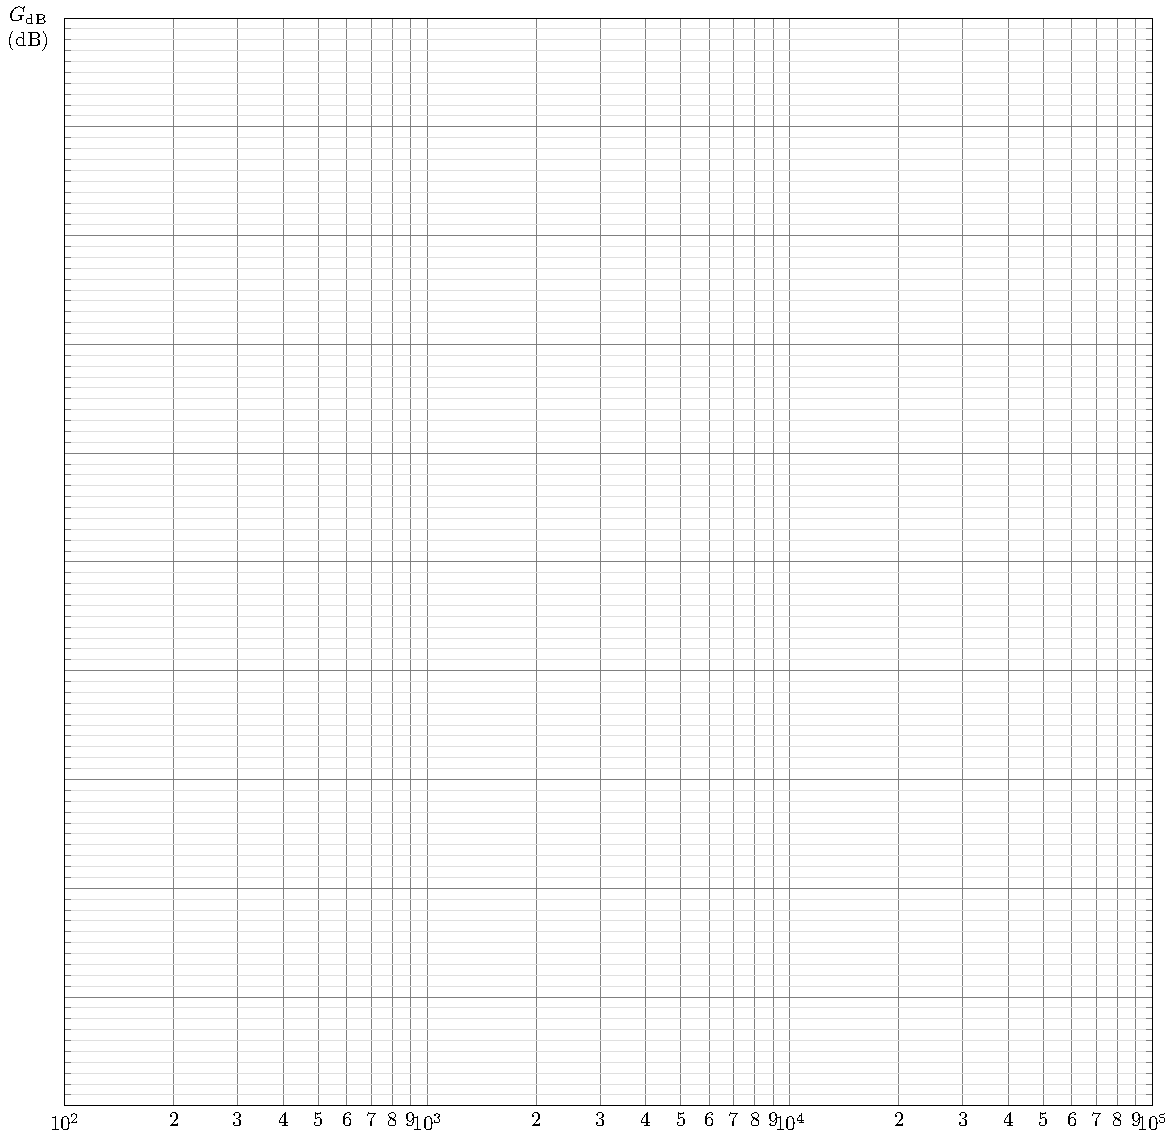
\includepdf{semilog}

\end{document}
